\appendix
\addtocontents{toc}{\protect\setcounter{tocdepth}{1}}% This turns off subsections
\chapter{Code Snippets}\label{ch:code-snippets}
Input types are presented within the brackets of each method and 
output types are presented after the \texttt{->} symbol. For example, in section \ref{code:SigmaProtocol}, 
the \texttt{first} method has the input:

\texttt{statement: \&Self::Statement, witness: \&Self::Witness, prover\_rng: \&mut R}

and the output: 

\texttt{(Self::State, Self::MessageA)}

\section{\texttt{SigmaProtocol Interface}}
\label{code:SigmaProtocol}
\begin{lstlisting}[language=rust]
  fn first<R: CryptoRngCore>(
      statement: &Self::Statement,
      witness: &Self::Witness,
      prover_rng: &mut R,
  ) -> (Self::State, Self::MessageA)
  where
      Self: Sized;

  fn second<R: CryptoRngCore>(verifier_rng: &mut R) -> Self::Challenge
  where
      Self: Sized;

  fn third<R: CryptoRngCore>(
      statement: &Self::Statement,
      state: Self::State,
      witness: &Self::Witness,
      challenge: &Self::Challenge,
      prover_rng: &mut R,
  ) -> Self::MessageZ
  where
      Self: Sized;

  fn verify(
      statement: &Self::Statement,
      a: &Self::MessageA,
      c: &Self::Challenge,
      z: &Self::MessageZ,
  ) -> bool
  where
      Self: Sized;
\end{lstlisting}

\section{\texttt{HVzk} \& \texttt{EHVzk} Interface}
\label{code:hvzk}

\begin{lstlisting}[language=rust]
  /// Honest-Verifier Zero Knowledge
  pub trait HVzk: SigmaProtocol {
      fn simulate(
          statement: &Self::Statement,
      ) -> (Self::MessageA, Self::Challenge, Self::MessageZ);
  }

  /// Extended Honest-Verifier Zero Knowledge
  pub trait EHVzk: SigmaProtocol {
      fn simulate(
          statement: &Self::Statement,
          challenge: &Self::Challenge,
          z: &Self::MessageZ,
      ) -> Self::MessageA;
  }
\end{lstlisting}

\section{Schnorr's Protocol}\label{code:schnorr}
\lstinputlisting[language=rust]{code/schnorr.txt}

\section{CDS94 Compiler: \texttt{SelfCompiler}}\label{code:cds}
\lstinputlisting[language=rust]{code/cds.txt}

\section{Stacking Sigmas Compiler: \texttt{SelfStacker}}\label{code:stacksig}
\lstinputlisting[language=rust]{code/stacksig.txt}

\section{Test Example: CDS94 Tests}\label{code:cds-tests}
\lstinputlisting[language=rust]{code/cds_tests.txt}

\chapter{Progress Report}
\section{Introduction}

Zero-Knowledge proofs \cite{GMR85} are protocols that allow a prover to convince a verifier that an NP statement is true, while revealing no additional information except the validity of their assertion. Early research proved that all languages in NP have zero-knowledge proof systems \cite{DBLP:conf/focs/GoldreichMW86}, and recent results have provided more efficient zero-knowledge proofs that are being used in practice. 

In many cases, it is desirable to have a zero-knowledge proof for a disjunctive statement, which is an NP statement with a set of clauses that are connected with logical ORs. Disjunctive statements have very useful properties that occur commonly in practice, such as proving ones membership to a particular group, or showing the existence of a bug in a verifier's code base \cite{StackedGF}. Zero-knowledge becomes an important property in cases where revealing the exact clause (or clauses) that is true may reveal private information about the prover, such as their identity. A long line of research has focussed on how $n$ zero-knowledge proofs, each for one statement, can be composed into a new zero-knowledge proof of the disjunction of these statements. 

In their 1994 paper, Cramer, Damg{\aa}rd, and Schoenmakers \cite{CDS94} provide a generic compiler to compose 3-round public coin proofs of knowledge, or more succinctly (and more popularly) known as $\Sigma$-protocols. %perhaps discuss more
More recently, Goel {\em et al.} \cite{StackingSigmas} improved on this further, providing a generic compiler for a large class of $\Sigma$-protocols and also reducing the size of the resulting proof. 

While extensive research has been conducted, there is a lack of notable real-world implementations of these results
\footnote{It should be noted that Hall-Andersen \cite{MHAStackSig} has provided a benchmark of applying the compiler in \cite{StackingSigmas} to Schnorr's discrete log protocol \cite{Schnorr}.}. This project seeks to build upon their work by implementing the compilers described in \cite{CDS94} and \cite{StackingSigmas}. Once implemented, we aim to provide a benchmark for both protocols to explore and measure how they differ. This will hopefully provide some valuable insights as to how these designs perform in practice, which may in turn lead to further improvements in the future that may have a broad impact on existing and upcoming cryptographic systems that rely on such a use case. 

\subsection{Related work}
\label{sec:related_work}
As part of their work in \cite{StackingSigmas}, Hall-Andersen provides an implementation of the Stacking Sigmas (SS) compiler \cite{MHAStackSig}. In this implementation, they apply the SS compiler to Schnorr over Ristretto25519 to obtain efficient ring signatures from discrete log and random oracles. 

% Stacked Garbling implementation
\section{Background}
\label{sec:background}

\subsection{Disjunctive Zero-Knowledge}

\begin{definition}[NP Relations]
Let $R \subseteq \{0,1\}^* \times \{0,1\}^*$ be a binary relation. Then $w(x) = \{w \mid (x,w) \in R\}$ and $L_R = \{x \mid \exists w, (x,w) \in R\}$. If $(x,w) \in R$, we say that $w$ is a witness for $x$. $R$ is an NP-relation if it fulfils the following two properties:
\begin{enumerate}
    \item \textbf{Polynomially bounded.} We say that $R$ is \textit{polynomially bounded} if there exists a polynomial $p$ such that $|w| \le p(|x|), \forall (x,w) \in R$. 
    \item \textbf{Polynomial-time verification.} There exists a polynomial-time algorithm for deciding membership in $R$. Consequently, $L_R \in NP$. 
\end{enumerate}

Throughout this document, we will use $\mathcal R$ to refer to a binary NP-relation.
\end{definition}

\begin{definition}[Zero-Knowledge]
A proof or argument system $(P,V)$ is zero-knowledge over $\mathcal R$ if there exists a \textit{probabilistic polynomial time} (PPT) simulator $\mathcal S$, such that for all $(x,w) \in R$, the distribution of the output $\mathcal S(x)$ of the simulator is indistinguishable from $\ViewPV$, which denotes the distribution over transcripts generated by the interaction of $P$ and $V$ within the proof or argument system.
\end{definition}

Intuitively, this means that $V$ should not learn anything from the transcripts  with $P$ that they cannot already learn on their own by running the simulator $\mathcal S$; they learn nothing new.

\begin{definition}[Disjunctive Zero-Knowledge]
Given a sequence of statements $(x_1,x_2,\ldots, x_l)$, a \textit{disjunctive zero-knowledge proof} is a protocol to prove in zero-knowledge that $x_1 \in \mathcal L_1 \lor x_2 \in \mathcal L_2 \lor \ldots \lor x_l \in \mathcal L_l$, for NP languages $\mathcal L_i$. We term clauses for which the prover has a witness for as \textit{active} clauses. 
\end{definition}

\begin{definition}[Honest-Verifier Zero-Knowledge]
A proof system is \textit{honest-verifier zero-knowledge} if it only requires that $\mathcal S$ is an efficient simulator for honest (non-malicious) probabilistic polynomial time verifier strategies $V$. If $V$ is malicious then the distribution of the output $\mathcal S(x)$ will no longer be indistinguishable from $\ViewPV$ for such proof systems. 
\end{definition}

\subsection{$\Sigma$-protocols}
\begin{definition}[$\Sigma$-Protocol]
Let $\mathcal R$ be an NP relation. A $\Sigma$-protocol $\Pi = (A, Z, \phi)$ for $\mathcal R$ is a 3-round protocol between a prover algorithm $P$ and a verifier algorithm $V$. Conversations between $P$ and $V$ are ordered triples of the form $(a,c,z)$, and are known as \textit{transcripts}. The protocol consists of a tuple of probabilistic polynomial time algorithms $(A, Z, \phi)$ with the following interfaces:
\begin{itemize}
    \item $a \leftarrow A(x,w; r^p)$ : Given statement $x$, witness $w \in w(x)$, and prover randomness $r^p$ as input; output the first message $a$ that $P$ sends to $V$ in the first round. 
    \item $c \samplefrom \{0,1\}^\kappa$: $V$ samples a random challenge $c$ and sends it to $P$ in the second round. 
    \item $z \leftarrow Z(x,w,c; r^p)$: Given $x$, $w$, $c$, and $r^p$ as input; output the message $z$ that $P$ sends to $V$ in the third round.
    \item $b \leftarrow \phi(x,a,c,z)$: Given $x$, and the messages in the transcript, output a bit $b \in \{0,1\}$. This algorithm is executed by $V$, and $V$ accepts if $b = 1$.
\end{itemize}
A $\Sigma$-protocol has the following properties:
\begin{enumerate}
    \item \textbf{Completeness.} $\Pi$ is complete if for any $x$, $w \in w(x)$, and any prover randomness $r^p \samplefrom \{0,1\}^\lambda$, the following holds:
    \begin{gather*}
        Pr\left[\phi(x,a,c,z) = 1 \st a \leftarrow A(x,w;r^p); c\samplefrom \{0,1\}^\kappa; z \rightarrow Z(x,w,c;r^p)\right] = 1
    \end{gather*}
    \item \textbf{Special Soundness.} $\Pi$ is said to have special soundness if  there exists a PPT extractor $\mathcal E$, such that given any two transcripts $(a,c,z)$ and $(a,c',z')$ for statement $x$, where $c \ne c'$ and $\phi(x,a,c,z) = \phi(x,a,c',z') = 1$, an element of $w(x)$ can be computed by $\mathcal E$.
    \item \textbf{Special Honest-Verifier Zero-Knowledge.} $\Pi$ is SHVZK if there exists a PPT simulator $\mathcal S$, such that for any $x$, $w$, $(x,w) \in \mathcal R$, the distribution over the output $\mathcal S(x, c^*)$ is indistinguishable from the distribution over transcripts produced by the interaction between $V$ and $P$ when the challenge is $c^*$.
    \begin{multline*}
        \{(a, z) \mid c^* \samplefrom \{0,1\}^\kappa; (a,z) \leftarrow \mathcal S(1^\lambda,x,c^*)\} 
        \approx_{c^*} \\
        \{(a,z) \mid r^p \samplefrom \{0,1\}^\lambda; a \leftarrow A(x,w;r^p); c^* \samplefrom \{0,1\}^\kappa; z \leftarrow Z(x,w,c^*;r^p)\}
    \end{multline*}
    
\end{enumerate}


\end{definition}



Explain transcripts, witness indistinguishable and WH protocols. Explain HVZK and SHVZK?

\subsection{Schnorr's Identification Protocol}
There are two parties in an \textit{identification scheme}, the prover $P$ and the verifier $V$, and the objective of the protocol is for the prover to convince the verifier that they are who they claim to be. More precisely, $V$ is convinced that $P$ knows the private key that corresponds to the public key of $P$. A familiar example is the standard protocol of password authentication.

Schnorr's protocol \cite{Schnorr} is an identification scheme where $P$ proves knowledge of the discrete log $x$ of a group element $H \in \G$, where $H = x \cdot G$ for some generator $G \in \G$. $(\G, +)$ is a finite abelian group with $+$ as the binary operator\footnote{We have chosen to define $\G$ with the $+$ operator because our implementation uses elliptic curves which are finite abelian groups over addition. The discrete log can be defined equivalently with multiplication like so: $h = g^x$}. The protocol relies on the assumption that finding $x$ given only $H$ and $G$ is computationally difficult -- this is not always the case. The hardness of finding the discrete log depends on the choice of group $\G$ (cite some resource or elaborate). Conversely, proving that $H = x \cdot G$ given $x$ and $G$ can be computed efficiently. 

In our implementation, we plan to use the Ristretto group \cite{ristretto_web}: a construction of a prime order group from a family of elliptic curves known as Edwards curves \cite{Edwards2007}. 

\begin{definition}[Schnorr's Protocol \cite{Schnorr}]
Let $\G = E(\F_q)$, where $E$ is an elliptic curve over the finite field $\F_q$. Suppose that both the prover $P$ and verifier $V$ agree on $E$ and $\F_q$, then let $H \in E(\F_q)$ be the public key that corresponds to the private key $x$ such that $H = x \cdot G$. The prover convinces the verifier that they have knowledge of the private key by doing the following:

\begin{enumerate}
    \item $P$ generates random $r \in \F_q$, and computes the point $U = r \cdot G$. $P$ sends the point $U$ to $V$.
    \item $V$ computes a random $c \in \F_q$, and sends $c$ to the $P$.
    \item $P$ computes $z = (r + c \cdot x_P) \mod n$, and sends $z$ to the $V$.
    \item $V$ checks that $z \cdot G = U + c \cdot H$.
\end{enumerate} 

Evaluating the final equation, we can easily see that $V$ accepts if and only if $x = x_P$. 

\begin{equation*}
    z \cdot G = U + c \cdot H \iff
    r \cdot G + c \cdot x_P \cdot G  = r \cdot G + c \cdot x \cdot G \iff
    x  =  x_P
\end{equation*}
\end{definition}


\textbf{A simulator for Schnorr's protocol.} We construct a simulator for Schnorr's protocol by running it "in reverse":

\begin{center}
    \begin{problem}[]{Let our simulator be $S(H)$}
    $z \randselect \F_q$ ($\randselect$ = select randomly from)
    
    $c \randselect \F_q$
    
    $U = z \cdot G - c \cdot H$
    \tcblower
    \textbf{output} $(U,c,z)$
    \end{problem}
\end{center}

Since $z$ and $c$ are both chosen randomly, the resulting $U$ is also random, and our output will have the same distribution as the distribution over transcripts in an actual interaction.

\subsection{Shamir's Secret Sharing Scheme}
A \textit{secret sharing scheme} is a method of distributing a secret $s$ to $n$ participants in a way that no one participant has intelligible information about the secret. This is achieved by splitting up $s$ into \textit{shares}, distributing one share to each participant in a way that a subset of participants can reconstruct $s$. Subsets that can reconstruct the secret are called \textit{qualified sets}. For \textit{perfect} secret sharing schemes, like Shamir's, participants in the complement \textit{non-qualified} sets cannot obtain any information about the secret.

Shamir's secret sharing scheme \cite{DBLP:journals/cacm/Shamir79} is also what is known as a \textit{threshold sharing scheme}. These are schemes that produce  qualified sets of size $d$. Any $d$ out of $n$ participants can reconstruct the secret; with $d-1$ shares and less, no  information about the secret can be obtained. 

\subsection{CDS94 Compiler}


In our implementation, we will use Schnorr's discrete log protocol over Ristretto25519 and Shamir's secret sharing scheme to demonstrate the compilation of $\Sigma$-protocol into a $\Sigma$-protocol for the disjunction of $n$ statements. 

We will attempt to make the implementation as general as possible to open up for the future possibility to take any $\Sigma$-protocol that suits our requirements and transform it disjunctive zero-knowledge $\Sigma$-protocol.

\subsubsection{The Witness Indistinguishable (WI) compilation}

In their paper, Cramer {\em{et al}} \cite{CDS94} presents 2 primary ways to construct a WI protocol from a $\Sigma$-protocol $\mathcal P$ (Theorem 8 and 9). 

\begin{itemize}
    \item Theorem 8 requires a smooth secret sharing scheme, and a HVZK $\Sigma$-protocol, while
    \item Theorem 9 requires special honest-verifier ZK (SHVZK) with at least a semi-smooth secret sharing scheme.
\end{itemize}

Since, SSS is a smooth threshold secret sharing scheme (required for 8), and Schnorr's protocol is SHVZK (required for 9), we can choose either construction. 
\textit{We will use \textbf{Theorem 8} in this project.}

\textbf{Theorem 8 \cite{CDS94}}. Given $\mathcal P$, $R_\Gamma$, $\Gamma$, and $\mathcal S(k)$ where

\begin{itemize}
    \item $\mathcal P$ is a 3-round public coin ($\Sigma$-protocol) HVZK proof of knowledge for relation $R$, which satisfies the special soundness property.
    \item $\Gamma = \{ \Gamma(k) \}$ is a family of monotone access structures
    \item $\{\mathcal S(k)\}$ is a family of smooth secret sharing schemes such that the access structure of $\mathcal S(k)$ is $\Gamma(k)^*$
    \item $R_\Gamma$ is a relation where $((x_1,\ldots,x_m),(w_1,\ldots,w_m)) \in R_\Gamma$ if and only if ($\iff$)
    \begin{itemize}
        \item all $x_i$'s are of the same length $k$, and 
        \item the set of indices $i$ for which $(x_i,w_i) \in R$ corresponds to a qualified set in $\Gamma(k)$
    \end{itemize}
\end{itemize}

Then, there exists a $\Sigma$-protocol that is witness indistinguishable for the relation $R_\Gamma$. (The proof of Theorem 8 and 9 is given in their paper.)

\subsubsection{Protocol Description}
Let $A \in \Gamma$ denote the set of indices $i$ for which our prover $P$ knows a witness for $x_i$

\begin{enumerate}
    \item For each $i \in \bar A$, $P$ runs a simulator on input $x_i$ to produce transcripts of conversations in the form $(m_1^i, c_i, m_2^i)$.
    \begin{itemize}
        \item For each $i \in A$, $P$ inputs the witness $w_i$ for $x_i$ to $\mathcal P$ and takes what the prover $P^*$ in $\mathcal P$ sends as $m_1$ as $m_1^i$.
        \item Essentially we take the return value of the first round of $\mathcal P$ as our message $m_1^i$.
        \item Finally, $P$ sends all $m_1^i$ to $V$, where $i = 1, \ldots, n$
    \end{itemize}
    \item $V$ chooses a $t$-bit string $s$ at random and sends it to $P$
    \item $P$ forms challenges $c_i$ for $i \in A$, such that $share(c_i) \cup \{share(c_j)|j \in \bar A\}$ is a qualified set in $\Gamma$ consistent with $s$.
    \begin{itemize}
        \item For $i \in A$, $P$ uses it's knowledge of $w(x_i)$ to compute a valid $m_2^i$ for $(m_1^i, c_i)$ by running the prover's algorithm in $\mathcal P$.
        \item $P$ then sends $c_i, m_2^i$ for $i = 1 ,\ldots, n$ to $V$. 
    \end{itemize}
    \item $V$ checks that all conversations $(m_1^i, c_i, m_2^i)$ would lead to acceptance by the verifier in $\mathcal P$
    \begin{itemize}
        \item During this process, $V$ checks that $share(c_i)$ is consistent with secret $s$.
        \item Accept if all true, otherwise reject. 
    \end{itemize}
\end{enumerate}


\section{Progress}
\label{sec:progress}

\subsection{CDS94 Compiler}
In this implementation of the compiler, we will use 

\begin{itemize}
    \item the elliptic curve version of Schnorr's discrete log protocol as our $\Sigma$-protocol, and
    \item Shamir's secret sharing scheme (SSS)
\end{itemize}

to demonstrate the compilation of $\Sigma$-protocol into a disjunctive/threshold $\Sigma$-protocol for $n$ statements. 

We will attempt to make the implementation as general as possible to open up for the future possibiity to take any $\Sigma$-protocol that suits our requirements and transform it into a $\Sigma$-protocol for $n$ statements.  

\subsubsection{The Witness Indistinguishable (WI) compilation}

In their paper, Cramer {\em{et al}} presents 2 primary ways to construct a WI protocol from a $\Sigma$-protocol $\mathcal P$ (Theorem 8 and 9). 

\begin{itemize}
    \item Theorem 8 requires a smooth secret sharing scheme, and a HVZK $\Sigma$-protocol, while
    \item Theorem 9 requires special honest verifier ZK (SHVZK) with at least a semi-smooth secret sharing scheme.
\end{itemize}

Since, SSS is a smooth threshold secret sharing scheme (required for 8), and Schnorr's protocol is SHVZK (required for 9), we can choose either construction. 
\textit{We will use \textbf{Theorem 8} in this project.}

\textbf{Theorem 8}. Given $\mathcal P$, $R_\Gamma$, $\Gamma$, and $\mathcal S(k)$ where

\begin{itemize}
    \item $\mathcal P$ is a 3-round public coin ($\Sigma$-protocol) HVZK proof of knowledge for relation $R$, which satisfies the special soundness property.
    \item $\Gamma = \{ \Gamma(k) \}$ is a family of monotone access structures
    \item $\{\mathcal S(k)\}$ is a family of smooth secret sharing schemes such that the access structure of $\mathcal S(k)$ is $\Gamma(k)^*$
    \item $R_\Gamma$ is a relation where $((x_1,\ldots,x_m),(w_1,\ldots,w_m)) \in R_\Gamma$ if and only if ($\iff$)
    \begin{itemize}
        \item all $x_i$'s are of the same length $k$, and 
        \item the set of indices $i$ for which $(x_i,w_i) \in R$ corresponds to a qualified set in $\Gamma(k)$
    \end{itemize}
\end{itemize}

Then, there exists a $\Sigma$-protocol that is witness indistinguishable for the relation $R_\Gamma$. (The proof of Theorem 8 and 9 is given in their paper.)

\subsubsection{Protocol Description}
Let $A \in \Gamma$ denote the set of indices $i$ for which our prover $P$ knows a witness for $x_i$

\begin{enumerate}
    \item For each $i \in \bar A$, $P$ runs a simulator on input $x_i$ to produce transcripts of conversations in the form $(m_1^i, c_i, m_2^i)$.
    \begin{itemize}
        \item For each $i \in A$, $P$ inputs the witness $w_i$ for $x_i$ to $\mathcal P$ and takes what the prover $P^*$ in $\mathcal P$ sends as $m_1$ as $m_1^i$.
        \item Essentially we take the return value of the first round of $\mathcal P$ as our message $m_1^i$.
        \item Finally, $P$ sends all $m_1^i$ to $V$, where $i = 1, \ldots, n$
    \end{itemize}
    \item $V$ chooses a $t$-bit string $s$ at random and sends it to $P$
    \item $P$ forms challenges $c_i$ for $i \in A$, such that $share(c_i) \cup \{share(c_j)|j \in \bar A\}$ is a qualified set in $\Gamma$ consistent with $s$.
    \begin{itemize}
        \item For $i \in A$, $P$ uses it's knowledge of $w(x_i)$ to compute a valid $m_2^i$ for $(m_1^i, c_i)$ by running the prover's algorithm in $\mathcal P$.
        \item $P$ then sends $c_i, m_2^i$ for $i = 1 ,\ldots, n$ to $V$. 
    \end{itemize}
    \item $V$ checks that all conversations $(m_1^i, c_i, m_2^i)$ would lead to acceptance by the verifier in $\mathcal P$
    \begin{itemize}
        \item During this process, $V$ checks that $share(c_i)$ is consistent with secret $s$.
        \item Accept if all true, otherwise reject. 
    \end{itemize}
\end{enumerate}

Requirements
Schnorr
- Have a simulator we can call publically
- Compiler will interface through protocol (can't access prover directly(?))
- Function for each round of protocol

SSS
 - If we have $n$ statements, and we want $P$ to prove that they know $d$ out of $n$ we have to use SSS with threshold $n-d+1$.
 - API for qualified set completion.


\section{Project management}

Discuss why we switch from Notion to using GitHub Projects. 

Discuss why we change from plan-based to agile development. 

Present timetable/plan for term 2. Mention extension to SNARKS.

Outline risk management plan. Explain why we have not conducted all research necessary, such as for Stacking Sigmas and SNARKS. Explain that Stacking Sigmas is much more complicated and work on CDS is required to familiarise with the cryptographic concepts. Explain that it is an ideal plan that is possible, but there are also likely to be unexpected issues and we have plan B. 



\chapter{Hardware Specification}
\label{sec:hardware-spec}
\lstinputlisting[]{../assets/hardware-specs.txt}


\chapter{Threat Model}
\label{sec:threat-model-appendix}
\section{Overview}

\begin{figure}[h]
    \centering
    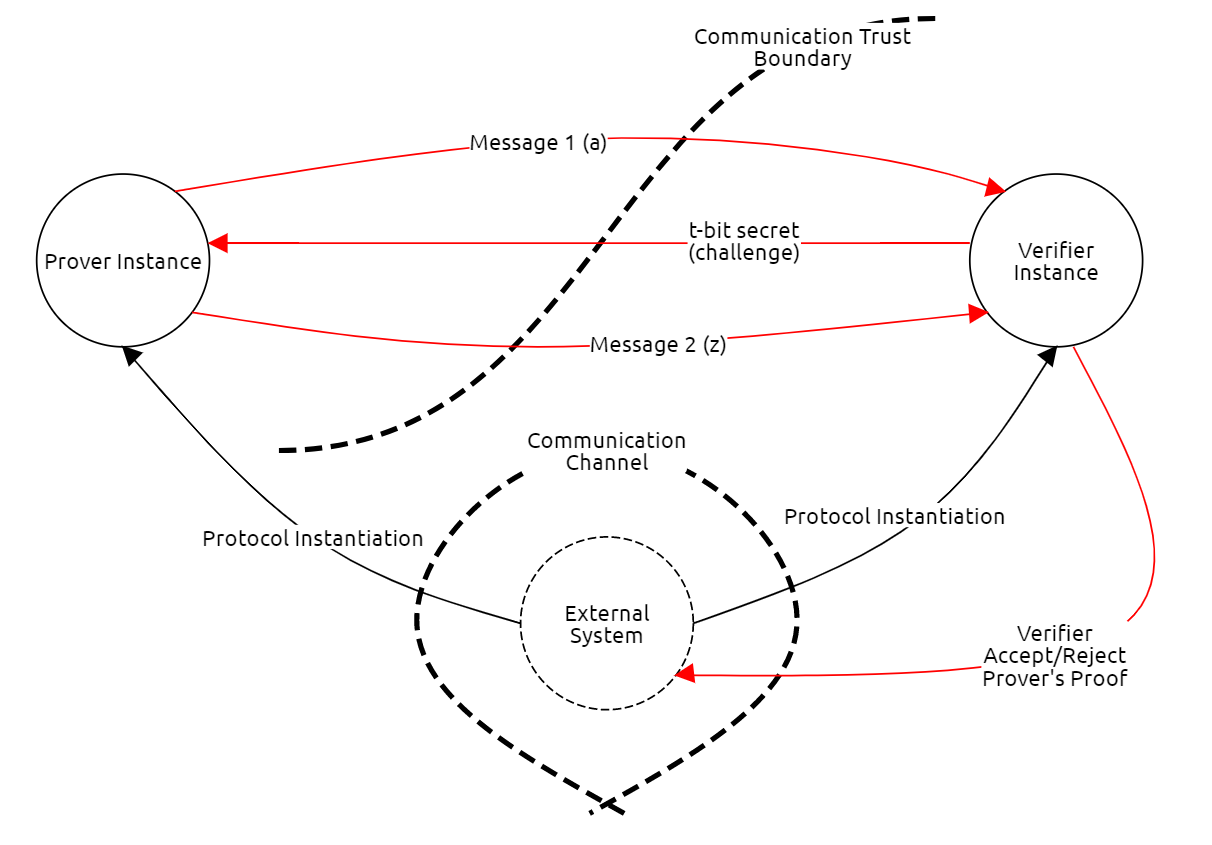
\includegraphics[width=\linewidth]{../assets/threat-model.png}
    \caption{Threat Model Diagram}
    \label{fig:threat_model}
\end{figure}

There should be no known way for adversaries to use the protocol in a way that it is not designed to. For example, under normal circumstances, the verifier should not have rewind access to a prover, this means that we will need to model state within the protocol and ensure that it is used properly (state-machine model). This should be a target of penetration tests. 


